\documentclass[a4paper]{article}
\usepackage[pdftex]{graphicx}
\usepackage[utf8]{inputenc}
\usepackage{enumerate}
\usepackage{amssymb}
\usepackage{icomma}
\usepackage{siunitx}
\sisetup{locale=DE} 
\usepackage{tikz}
\usepackage{href-ul}
\hypersetup{
	colorlinks=true,
	linkcolor=blue,
	urlcolor=blue}
\usepackage{geometry}
\geometry{a4paper, top=15mm, left=15mm, right=15mm, bottom=15mm,
	headsep=10mm, footskip=12mm}

\begin{document}
	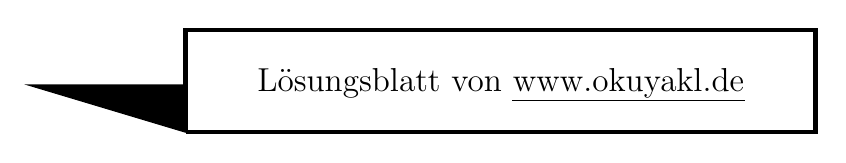
\begin{tikzpicture}(10,3)
		\draw[ultra thick](2,0) --(10,0) -- (10,1.3) --(2,1.3) -- (2,0);
		\draw[fill=black](2,0)-- (0,.6) -- (2,.6) -- (2,0);
		\node at (6,.6) {\large Lösungsblatt von \href{https://www.okuyakl.de}{www.okuyakl.de}};
	\end{tikzpicture}
	\vspace{0.5 cm}
	
	
{\bf Druck, Kraft und Arbeit}

\renewcommand{\arraystretch}{1.5}
\begin{tabular}{|p{1.4 cm}|p{1.4 cm}|p{1.4 cm}|p{1.4 cm}|p{1.4 cm}|}
	\hline
	& $\SI{}{\meter}$ & $\SI{}{\deci\meter}$ & $\SI{}{\centi\meter}$ & $\SI{}{\milli\meter}$\\
	\hline
	$\SI{1}{\meter}$ & 1 & 10 & 100 & 1000\\
	\hline
	$\SI{1}{\deci\meter}$ & 0,1 & 1 & 10 & 100\\
	\hline
	$\SI{1}{\centi\meter}$ & 0,01 & 0,1 & 1 & 10 \\
	\hline
	$\SI{1}{\milli\meter}$ & 0,001 & 0,01 & 0,1 & 1\\
	\hline
	
\end{tabular}
\hspace{0.5 cm}
\begin{tabular}{|p{1.4 cm}|p{1.4 cm}|p{1.4 cm}|p{1.4 cm}|}
	\hline
	& $\SI{}{\pascal}=\SI{}{\newton\over{\meter^2}}$ & $\SI{}{\kilo\pascal}$ & bar\\
	\hline
	$\SI{1}{\pascal}$ & 1 & 0,001 & $10^{-5}$\\
	\hline
	$\SI{1}{\kilo\pascal}$ & 1000  & 1 & 0,01\\
	\hline
	1 bar & $10^5$ & 100 & 1 \\
	\hline
\end{tabular}

\vspace{0.5 cm}
\begin{tabular}{|p{1.8 cm}|p{1.8 cm}|p{1.8 cm}|p{1.8 cm}|}
	\hline
	& $\SI{}{\meter^2}$ & $\SI{}{\deci\meter^2}$ & $\SI{}{\centi\meter^2}$ \\
	\hline
	$\SI{1}{\meter^2}$ & 1 & 100 & 10000\\
	\hline
	$\SI{1}{\deci\meter^2}$ & 0,01 & 1 & 100\\
	\hline
	$\SI{1}{\centi\meter^2}$ & 0,0001 & 0,01 & 1\\
	\hline
\end{tabular}
\hspace{0.5 cm}
\begin{tabular}{|p{1.8 cm}|p{1.8 cm}|p{1.8 cm}|}
	\hline
	&$\SI{}{\newton}$ & $\SI{}{\kilo\newton}$  \\
	\hline
	$\SI{1}{\newton}$ & 1 & 0,001\\
	\hline
	$\SI{1}{\kilo\newton}$ & 1000 & 1	\\
	\hline
\end{tabular}
\vspace{1 cm}

\renewcommand{\arraystretch}{2}
\begin{tabular}{|p{1,8 cm}|p{1.8 cm}|p{1.8 cm}|p{1.8 cm}|p{1.8 cm}|p{1.8 cm}|p{1.8 cm}|p{1.8 cm}|}
\hline
Kraft 1 & Fläche 1 & Weg 1 & Kraft 2 & Fläche 2 & Weg 2 & Druck & Arbeit \\ 
$F_1$ & $A_1$ & $s_1$ & $F_2$ & $A_2$ & $s_2$ & $p$ & $W$ \\
\hline
$\SI{12}{\newton}$ & $\SI{8}{\centi\meter^2}$ &$\SI{0,70}{\meter}$ &$\SI{2,4}{\kilo\newton}$ &$\SI{0,16}{\meter^2}$ & $\SI{3,5}{\centi\meter}$ &$\SI{15}{\kilo\pascal}$ &$\SI{8,4}{\joule}$ \\
\hline
$\SI{80}{\newton}$ & $\SI{30}{\centi\meter^2}$ &$\SI{0,60}{\meter}$ &$\SI{6,4}{\kilo\newton}$ &$\SI{0,24}{\meter^2}$ & $\SI{0,75}{\centi\meter}$ &$\SI{2,7}{\kilo\pascal}$ &$\SI{48}{\joule}$ \\
\hline
$\SI{1,4}{\newton}$ & $\SI{2,0}{\centi\meter^2}$ &$\SI{0,15}{\meter}$ &$\SI{7,0}{\newton}$ &$\SI{10}{\centi\meter^2}$ &$\SI{3,0}{\centi\meter}$ &$\SI{7,0}{\kilo\pascal}$ &$\SI{0,21}{\joule}$ \\
\hline
$\SI{0,20}{\kilo\newton}$ & $\SI{4,0}{\centi\meter^2}$ &$\SI{0,40}{\meter}$ &$\SI{10}{\kilo\newton}$ &$\SI{0,20}{\meter^2}$ &$\SI{8,0}{\milli\meter}$ &$\SI{0,50}{\mega\pascal}$ &$\SI{80}{\joule}$ \\
\hline
$\SI{5,2}{\newton}$ & $\SI{4,0}{\centi\meter^2}$ &$\SI{1,7}{\meter}$ &$\SI{26}{\newton}$ &$\SI{20}{\centi\meter^2}$ &$\SI{34}{\centi\meter}$ &$\SI{13}{\kilo\pascal}$ &$\SI{8,8}{\joule}$ \\
\hline
\end{tabular}
\vspace{0.5 cm}


\begin{center}
	\includegraphics[width=7 cm]{../../viecher/endcomic.pdf}
	
	Hier geht es zurück zum \href{https://www.okuyakl.de/phys/p9drkL076/aa076.pdf}{Aufgabenblatt}
\end{center}


\end{document}

